\input{/Users/daniel/github/config/preamble-por.sty}%available at github.com/danimalabares/config
%\input{/Users/daniel/github/config/thms-por.sty}%available at github.com/danimalabares/config

\newcommand{\rightlooparrow}{\mathbin{
    \vbox{\openup-10.25pt\halign{\hss$##$\hss\cr\circ\cr\longrightarrow\cr}}
}}

\begin{document}
\bibliographystyle{alpha}

\begin{minipage}{\textwidth}
	\begin{minipage}{1\textwidth}
		Topologia diferencial\hfill Daniel González Casanova Azuela
		
		{\small Prof. Vinicius Ramos\hfill\href{https://github.com/danimalabares/k3}{github.com/danimalabares/dt}}
	\end{minipage}
\end{minipage}\vspace{.2cm}\hrule

\vspace{10pt}
{\huge Topologia Diferencial}
\tableofcontents
\section{Aula 1}

\subsection{Plano do curso, bibliografia}

Cronograma
\begin{enumerate}
	\item[0.] Revisão de variedades.
	\item Transversalidade: Sard, top. forte, fraca, aproximação.
	\item  Teoria da interseção e indice.
	\item Teoria de Morse.
	\item Tópicos adicionais (possiveis): h-cobordismo, top. de baixa dimensão, Poincaré \(n\geq 5\).
\end{enumerate}

Bibliografía: \cite{milnordt} (intuição),  \cite{gui} (tranqui, tem muito), \cite{hirsch} (pesado, tem tudo, e importante ler, usa Análise Funcional). 

\subsection{Resumo da aula 1}

\begin{enumerate}
\item Revisão de vriedades, espaço topológico, 2-enumerável, 2-contável, Hausdorff, loc. euclidiano, dimensão é fixa nas componentes conexas, def. de carta, atlas, atlas \(C^k\), atlas maximal. \textbf{Obs.} Existem atlas que não contém sub atlas \(C^k\).
\item \textbf{Teorema.} \(k=1,\ldots, +\infty\) tuda \(C^k\)-variedade é  \(C^k\)-difeomorfa a uma \(C^\infty\)-variedade.
\item \textbf{Teorema.} \(1 \leq  \ell \leq  k \leq +\infty\), se \(M,N\) são \(C^k\)-variedades, \(C^\ell\)-difeomorfas, então \(M\) e $N$ são \(C^k\)-difeomorfas. {\color{2}No será \(\ell?\)}
\item \textbf{Partições da unidade}. Definição. \textbf{Exercício:} toda variedade topológica é paracompacta. \textbf{Teorema:} \(M\) variedade \(C^\infty\) e \(\{ U_i\}\) cobertura, então existe \(C^\infty\) partição da unidade subordinada. 
\end{enumerate}


\section{Aula 2}

\subsection{Lembre}

Dada uma variedade suave \(M\). Definimos como velocidades de curvas ou como derivações: \(T_pM\) é um espaço vetorial de dimensão $n$, onde para \(p \in U\), \((U, \varphi)\) carta, \(\varphi=(x^1,\ldots,x^n\) com base \(\left\{ \frac{\partial }{\partial x_1}\Big|_{p},\ldots,\frac{\partial }{\partial x^n}\Big|_{p} \right\} \). O \textit{\textbf{espaço cotangente}} é
\[T^*_p M=(T_pM)^* =\operatorname{Hom}(T_pM,\mathbb{R}).\]
A base dual é \(\left\{ dx^1|_{p},\ldots,dx^n|_{p} \right\} \) dada por
\[ dx^i|_{p}=\left(\frac{\partial }{\partial x^j}\right)\Big|_{p}=\delta_i^j=\begin{cases}
	1\qquad &\text{se } i=j \\
	0\qquad &\text{se não} 
\end{cases}\]

e ai extendemos por linearidade a todos os demais covetores.

\begin{remark}\leavevmode
	Note que mudando de carta a gente muda de base---não tem uma base canônica do espaço cotantente.
\end{remark}

\subsection{Fórmula de mudança de bases}

\begin{thing6}{Fórmula de mudança de bases}[Exercício]\leavevmode
\((U,\varphi),(V,\psi), p \in U \cap V\), \(\varphi=(x^1,\ldots,x^n\), \(\psi(y^1,\ldots,y^n\) com bases
\[\left\{ \frac{\partial }{\partial x_1}\Big|_{p},\ldots,\frac{\partial }{\partial x^n}\Big|_{p} \right\}, \qquad \left\{ \frac{\partial }{\partial y_1}\Big|_{p},\ldots,\frac{\partial }{\partial y^n}\Big|_{p} \right\},\]
mostre que
\[\frac{\partial }{\partial x^j}=\sum_{i=1}^n \frac{\partial y^i}{\partial x^j}\frac{\partial }{\partial y^i}\]

\end{thing6}

\subsection{Fibrado tangente}
\(M\) variedade,
\[TM:=\bigsqcup_{p \in M}T_pM.\]

Note que para toda carta \((U,\varphi)\) existe uma bijeção
\begin{align*}
	\phi^{-1}:U \times \mathbb{R}^n &\longrightarrow \pi^{-1}(U) \\
	\Big(p,(v_1,\ldots,v_n) \Big) &\longmapsto \sum_{i=1}^n v_i\frac{\partial }{\partial x^i}
\end{align*}
usando essa bijeção, topologizamos \(TM\). Mas ainda, induz uma estrutura de variedade topológica com cartas dadas pelas \(\phi\). Mas exatamente, as cartas são
\begin{align*}
	\phi_{(U,\varphi)}: \pi^{-1}(U) &\longrightarrow \varphi(U)\times\mathbb{R}^n \subset \mathbb{R}^{2n} \\
	\sum v_i \frac{\partial }{\partial x^i}\Big|_{p} &\longmapsto \Big(\varphi(p),(v_i) \Big)
\end{align*}
e a mudança de coordenadas também é \(C^\infty\), i.e. esa estrutura é diferenciável.

\begin{remark}\leavevmode
	Se variedade é \(C^k\), o fibrado tangente é \(C^{k-1}\).
\end{remark}

A gente vai fazer isso mesmo com o fibrado cotangente:
\[T^*  M= \bigsqcup_{p \in M} T^*_pM.\]
O mesmo procedimento mostra que \(T^* M\) é uma \(C^\infty\)-variedade de dimensão \(2n\).

\begin{remark}\leavevmode
	Para todo \(p \in M\) existe \(U \ni p\) vizinhança tal que \(\pi_1(U) \cong U \times \mathbb{R}^n\). {\color{2}Mas \(TM \not\cong M \times \mathbb{R}^n\) em geral}; nesse caso dizemos que \(M\) é \textit{\textbf{paralelizável}}.
\end{remark}

\begin{thing6}{Casos onde \(TM \cong M \times \mathbb{R}^n\)}\leavevmode
\begin{enumerate}
\item \(M \cong \mathbb{R}^n\), \(TM \cong \mathbb{R}^n \times \mathbb{R}^n\).
\item  \(M= S^1\), \(TS^1 \cong S^1 \times \mathbb{R}\).
\item  \(M\) 3-variedade orientável, então \(TM \cong M \times \mathbb{R}^3\). (Difícil mas verdadeiro.) \textbf{Hint.} Usando quaternios não é difícil obter uma base global.
\end{enumerate}
\end{thing6}

\subsection{Imersões e mergulhos}

Até agora definimos funções suaves, mas não o que é a diferencial delas.

\begin{defn}\leavevmode
	\(M,N\) variedades suaves e \(f:M \to N\) suave. A \textit{\textbf{derivada de $f$}} é
	\[Df_p:T_pM \to T_{f(p)}N,\]
uma aplicacão linear que pode ser definida usando a definição do espaço tangente de curvas ou de derivações. Se pensamos que \(v\) é uma clase de equivalência de curvas,
\(Df_p[\gamma]=[f \circ \gamma].\)
Se \(v: C^\infty(M) \to \mathbb{R}\) é uma derivação, a definição é o pus
rward
\begin{align*}
	Df_pv: C^\infty(N) &\longrightarrow \mathbb{R} \\
	(Df_pv)g &\longmapsto v(g \circ f).
\end{align*}
Tem outra forma de definir, que usando cartas coordenadas, onde \(Df_p\) está dada como uma matriz em termos das bases locais: em cartas \((U,\varphi),(V,\psi)\) de \(p\) e \(f(p)\), \(\varphi=(x^1,\ldots,x^n)\) e \(\psi=(y^1,\ldots,y^n)\). A notação fica
\[Df_p\left(\frac{\partial }{\partial x^j}|_{p}\right) =\sum_{i=1}^n\frac{\partial f_i}{\partial x^j}|_{p}\frac{\partial }{\partial y^i}|_{f(p)}\]
onde \(\frac{\partial f_i}{\partial x^j}\) é definida como
\[D(\psi \circ f \circ \varphi^{-1})_{ij}=\frac{\partial }{\partial x^j}(\psi \circ \varphi \circ \varphi^{-1})\]
\end{defn}

\begin{defn}\leavevmode
Seja \(f:M \to N\) uma função suave. \(f\) é uma \textit{\textbf{imersão em $p$}} se a derivada \(Df_p\) é injetiva. \(f\) é uma \textit{\textbf{submersão em $p$}} se \(Df_p\) é sobrejetiva. \(f\) é um \textit{\textbf{mergulho}} se é uma imersão injetiva tom inversa \(g:f(M) \to M\) contínua.
\end{defn}

\begin{example}\leavevmode
	O exemplo mas fácil é o caso das incusões em variedades produto:
	\begin{align*}
		M &\longrightarrow M \times N \\
		p &\longmapsto (p,q)
	\end{align*}
	E as projecões:
	\begin{align*}
		M \times N &\longrightarrow M \\
		(p,q) &\longmapsto p
	\end{align*}
	Outros exemplos de submersões são as projeções dos fibrados tangente e cotangente.
\end{example}

Para ver por que na definição de mergulho pedimos que a inversa seja contínua, considere o seguinte contraexemplo: \(\mathbb{R} \to \mathbb{R}^2\) uma curva que tem um ponto límite demais: a topologia no domínio é uma linha, mas a topologia no contradomínio e de um outro espaço, mas $f$ é um mergulho injetivo! A inversa de $f$ não é contínua (não manda limites em limites).

\begin{remark}\leavevmode
	Se \(f:M \to N\) é um mergulho, então \(f(M)\) herda uma estrutura de variedade diferenciável e $f$ é um difeomorfismo entre \(M\) e \(f(M)\).
\end{remark}

\begin{upshot}\leavevmode
	Merhulo são as treis condições que precisamos para que a imagem de $f(M)$ tenha estrutura diferenciável e \(f\) um difeomorphismo entre \(M\) e \(f(M)\). O lance é usar o teorema da função inversa. \(f(M)\) é chamada de uma \textit{\textbf{subvariedade}} de $N$.
\end{upshot}
Uma definição alternativa de \textit{\textbf{subvariedade}} é que para cada ponto \(p \in  Q \subset M\), \(Q\) subespaço topológico, existe uma carta de $N$ tal que \(\varphi(U \cap Q)=\mathbb{R}^k\). (Misha's). Tem uma terceira definição: \(Q\) é a imagem de um mergulho; para isso pode usar a inclusão como o mergulho.
In Misha's handouts:
\begin{thing4}{Exercise 2.23}\label{exer:2.23}\leavevmode
Let \(N_1,N_2\) be two manifolds and let \(\varphi_i:N_i\to M\) be smooth embeddings. Suppose that the image of \(N_1\) coincides with that of \(N_2\). Show that \(N_1\) and \(N_2\) are isomorphic.
\end{thing4}

\begin{thing5}{Remark 2.10}\leavevmode
By the above problem, in order to define a smooth structure on $N$, it sufficies to embed $N$ into \(\mathbb{R}^n\). As it will be clear in the next handout, every manifold is embeddable into \(\mathbb{R}^n\) (assuming it admits partition of unity). Therefore, in place of a smooth manifold, we can use ``manifolds that are smoothly embedded into \(\mathbb{R}^n\)".
\end{thing5}

\begin{thing3}{Notação}\leavevmode
Se \(f:M \to N\) é uma imersão escrevemos \(M \rightlooparrow N\), se é mergulho \(M \hookrightarrow N\) e se é submersão \(f: M \twoheadrightarrow N\).
\end{thing3}
Uma \textit{\textbf{subvariedade imersa}} é a imagem de uma imersão (que pode nem ser variedade…)

\begin{remark}\leavevmode
	\(Q \subset M\) subvariedade, então existe uma inclusão natural \(T_qQ \subset T_q M\) (linear injetiva) para todo \(q \in Q\). Claro, a derivada da inclusão \(\iota:Q \to M\), i.e. \(D\iota_q:T_qQ \to T_qM\).
\end{remark}
kj
Dado \(q \in Q\), existe \((U,\varphi)\) carta de \(M\) tal que \(\varphi|_{U \cap Q}\) é uma carta de \(Q\), é só botar a base \(\left\{\frac{\partial}{\partial x_1}\Big|_{p},\ldots,\frac{\partial}{\partial x^n}\Big|_{p}\right\}\) dentro da base de \(M\).

\subsubsection{Valores regulares}
\begin{defn}\leavevmode
	Seja \(f:M \to N\) \(C^\infty\), um ponto \(y \in N \) é dito \textit{\textbf{valor regular}} se $f$ é uma submersão em $x$ para todo \(x \in f^{-1}(y)\) i.e. \(Df_x\) é sobrejetiva para todo \(x \in f^{-1}(y)\).
\end{defn}

\begin{thm}[Do valor regular]\leavevmode
Se \(y \) é um valor regular de $f$, então \(f^{-1}(y)\) é uma subvariedade de \(M\) de dimensão \(\dim M- \dim N\). (Se \(f^{-1}(y)\neq \varnothing\).)
\end{thm}

\begin{remark}\leavevmode
	Isso é só outra encarnação do teorema da função implícita.
\end{remark}

\begin{proof}\leavevmode
\(x \in f^{-1}(y):=Q\). Pega cartas \(\varphi\) de $x$ e \(\psi\) de $y$. Supondo que \(f(U) \subset V\), e que \(x,y\) tem coordenadas 0.
\[\begin{tikzcd}
	U \subset M \arrow[r,"f"]\arrow[d,swap,"\varphi"]&  V \subset N\arrow[d, "\psi"]\\
	\mathbb{R}^m \arrow[ r, swap,"\Phi:\psi \circ f \circ \varphi^{-1}"]& \mathbb{R}^n
\end{tikzcd}\]
Note que \(\Phi(0)=0\) e que \(\Phi^{-1}(0)=\varphi(f^{-1}(y) \cap U)\).
\begin{claim}\leavevmode
	\(\Phi^{-1}(0)\) é uma subvariedade.
\end{claim}
Para tudo ficar claro vamos reescrever o teorema de função implícita.  \(\Phi'(0)\) é sobrejetiva. Temos que
\begin{align*}
	: \mathbb{R}^m &\longrightarrow \mathbb{R}^n \times \mathbb{R}^{m-n} \\
	z &\longmapsto \Phi(z)
\end{align*}
A ideia é que existe uma vizinhança \(W\) de \(0 \in \mathbb{R}^m\) e um difeomorfismo \(\eta:W \to W^{\smile}\) tal que
\begin{align*}
	\phi \circ \eta: W \subset \mathbb{R}^n \times \mathbb{R}^{m-n} &\longrightarrow \mathbb{R}^n \\
	(x_1,x_2) &\longmapsto x_1
\end{align*}
\end{proof}

\subsection{Fibrados vetoriais}
Um fibrado vetorial é uma coisa que generaliza os fibrados tangente e cotangente.
\begin{defn}\leavevmode
Sejam \(E, M\) variedades e \(\pi: E \to M\) submersão sobrejetiva. Dizemos que \(\pi\) é um \textit{\textbf{fibrado vetorial}} se para todo \(p \in M\), \(\pi^{-1}(p)=E_p\) possui uma estrutura de espaço vetorial tal que para todo \(p \in M\) existe \(U \ni p\) aberto e um difeomorfismo \(\varphi: \pi^{-1}(U) \to U \times \mathbb{R}^n\) tal que o seguinte diagrama comuta
\[\begin{tikzcd}
\pi^{-1}(U)\arrow[rr,"\varphi"]\arrow[dr,swap,"\pi"]&&U \times \mathbb{R}^n\arrow[dl,"\operatorname{pr}_1"]\\
&U
\end{tikzcd}\]
e
\[\varphi|_{E_p}:E_p \to \{ p\}\times \mathbb{R}^n\]
é um isomorfismo.
\end{defn}

\begin{example}\leavevmode
	\(TM,T^* M,TM \oplus  TM, TM \otimes TM, \Lambda^{k}(TM),\Lambda^{k}(T^*M),\operatorname{Sym}^k(TM)\).
\end{example}

\subsection{Seções}

\begin{defn}\leavevmode
	Uma \textit{\textbf{seção}} de \(\pi:E \to M\) é \(s:M \to E\) suave tal que \(\pi \circ s = \operatorname{id}\)
\[\begin{tikzcd}
E\arrow[d,"\pi",swap]\\
M \arrow[u, bend right,swap,"s"]
\end{tikzcd}\]
Uma seção de TM é uma função \(X: M \to TM\) tal que \(X(p) \in T_pM\), um \textit{\textbf{campo vetorial}}.
\end{defn}

\begin{thm}[da bola cabeluda]\leavevmode
\(M = S^{n}\), \(n\) par, \(X:M \to TM\) campo vetorial, então existe \(p \in M\) tal que \(X(p)=0 \in T_pM\).
\end{thm}

\begin{thing6}{Notação}\leavevmode
\(\Gamma(E) = \{ \text{seções de \(\pi:E \to M\)} \}\), \(\Gamma(TM)=\mathfrak{X}(M)\), \(\Gamma(T^*M)=\Omega^{1}(M)\), \(\Gamma(\Lambda^{k}(T^*M))=\Omega^{k}(M)\).

Para qualquer espaço vetorial \(V\),
\[\operatorname{Sym}^2(V^*)=\{f:V \times V \to \mathbb{R},\text{ bilinear, }f(x,y)=f(y,x) \}\subset V^* \otimes V^*.\]
E para fibrado vetorial \(E\),
 \[\operatorname{Sym}^2(E)=\bigsqcup_{p \in M}\operatorname{Sym}^2(E^*_p).\]
\end{thing6}

\begin{defn}\leavevmode
	Uma \textit{\textbf{métrica Riemanniana}} em \(E\) é uma seção \(s: M \to \operatorname{Sym}^2(E)\) tal que \(s(p):E_p \times E_p \to \mathbb{R}\) é positiva definida, i.e. \(s(p)(x,x)>0\) se \(x \neq  0\).
\end{defn}

\begin{remark}[Aprox.]\leavevmode
	Todo fibrado vetorial tem uma métrica Riemanniana: usando a métrica euclidiana dada em cada carta, usamos uma partição da unidade para extender a uma seção global, somar e notar que fica positiva definida.
\end{remark}

É muito fácil construir seções do fibrado cotangente: para \(f \in C^\infty(M)\), a diferencial \(df :M \to T^*M\) é uma seção do fibrado cotangente, i.e. \(df \in \Gamma(T^*M)\) porque
\[df_p=Df_p:T_pM \to T_{f(p)}\mathbb{R}\]

\begin{exercise}\leavevmode
	Qualquer seção é um mergulho de \(M\) em \(E\).
\end{exercise}

\begin{thing6}{Mais uma}\leavevmode
$g$ uma métrica Riemanniana em \(TM\).
\[g_p:T_pM \times T_p M \to \mathbb{R}\]

\begin{align*}
	g_p^\sharp :T_pM &\longrightarrow  T^*_pM\\
	v &\longmapsto g(v,\cdot)
\end{align*}
Então o \textit{\textbf{gradiente}} de \(f\) é
\[(g^\sharp _p)^{-1}(df_p):=\operatorname{grad}_pf\]
\end{thing6}

\section{Aula 3: Teorema de Sard}

\subsection*{Teorema da função implícita (aula pasada)}

Uma função \(f:\mathbb{R}^n \to \mathbb{R}^m\) suave tal que \(f(0)=0\) e  \(f'(0)\) é sobrejetiva (\(\implies n \geq m\)). Então existe uma vizinhança de \(0 \in \mathbb{R}^n\) \(U\) e \(\tilde{U}\) \textbf{e um difeomorfismo} \(\varphi: U \to \tilde{U}\) tal que
\begin{align*}
	f \circ \varphi: \mathbb{R}^m \times \mathbb{R}^{n-m} &\longrightarrow \mathbb{R}^m \\
	(x,y) &\longmapsto x
\end{align*}

\begin{proof}\leavevmode
Parecido como a prova de \cite{tus} no teorema do valor regular, usando uma matrix com um \(*\), a identidade, e uma matriz invertível.
\end{proof}

\subsection{Transversalidade: Teorema de Sard}

A prova do teorema de Sard é muito técnica. Porém, a parte difícil é só análise em \(\mathbb{R}^n\).

Pegue \(a=(a_1,\ldots,a_n),b=(b_1,\ldots,b_n) \in \mathbb{R}^n\), defina um \textit{\textbf{cubo}} como sendo
\[c(a,b)=\prod_{i=1}^n ]a_i,b_i[ \subset \mathbb{R}^n.\]
Note que \(\operatorname{Vol}(a,b)=\prod_{i=1}^n(b_i-a_i).\)

\begin{thing5}{What \cite{lee} does}\leavevmode
\begin{enumerate}
\item A compact subset whose intersection with every hyperplane has measure zero has measure zero.
\item Graph of continuous function has measure zero.
\item Affine subspaces of \(\mathbb{R}^n\) have measure zero.
\item \textbf{Smooth map maps measure zero to measure zero.} 
\item A set in a manifold has \textit{\textbf{measure zero}} if it(s intersection with the respective domain) is mapped to a set of measure zero by any chart.
\item Confusing lemma.
\item Complement of zero measure is dense (in manifolds).
\item Smooth map \textit{of manifolds} maps measure zero to measure zero.
\item Sard's theorem (heavy proof): critical value set of smooth map has measure zero.
\item Corollary \textbf{(minisard)}: image of smaller dimension manifolds under smooth map has measure zero. Corollary 2: smaller dimension immersed submanifolds have measure zero.
\item Up next: Whitney embedding theorem.
\end{enumerate}
\end{thing5}

\begin{defn}\leavevmode
	\begin{figure}[H]
		\centering
		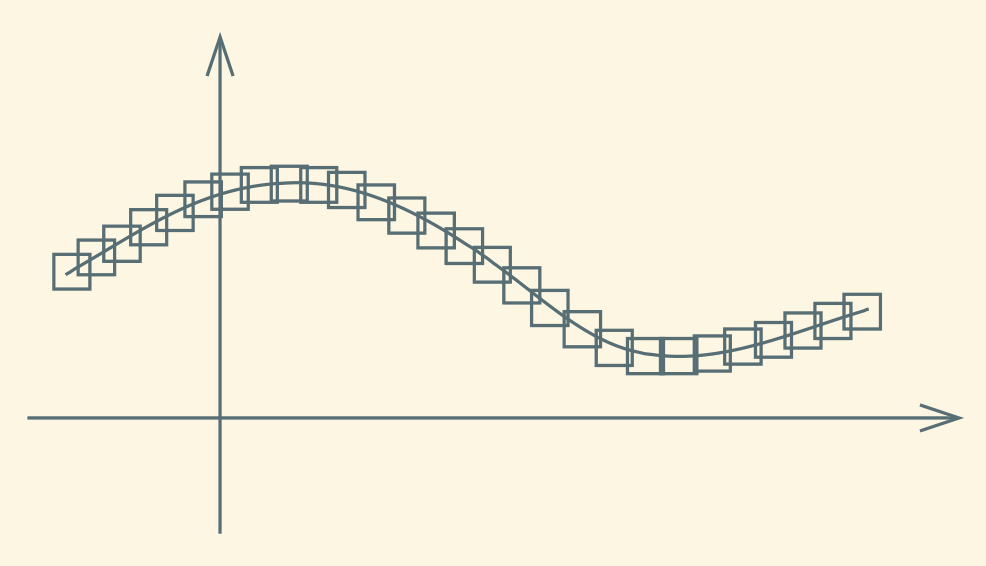
\includegraphics[width=0.7\textwidth]{fig1}
	\end{figure}
\(S \subset \mathbb{R}^n\) possui \textit{\textbf{medida nula}} se \(\forall  \varepsilon >0\) existe \(\{c_i\}_{i=1}^\infty\) cubos (ou bolas) tais que \[S \subset \bigcup_{i=1}^\infty \operatorname{Vol}(c_i)<\varepsilon\]
\end{defn}

\begin{prop}\leavevmode
	\begin{enumerate}
	\item Uma união enumerável de conjuntos de medida nula tem medida nula.
	\item \(f : \mathbb{R}^n \to \mathbb{R}^n\) \(C^1\) e \(S \subset \mathbb{R}^n\) tem medida nula, então \(f(S)\) tem medida nula.
	\end{enumerate}
\end{prop}

\begin{proof}\leavevmode
\begin{enumerate}
\item \(\{S_i\}\) enumerável de medida nula, para cada $i$ você pode escolher cubos \(C^i_1,C^i_2,\ldots\) que cobren \(S_i\) e tal que a soma dos volumes deles é menor do que \(\sum_j \operatorname{Vol}(C^i_j)<\frac{\varepsilon}{2^i}\). Vai ver que a soma dos volumeis variando tanto \(i\) como \(j\) da \(\varepsilon\).

\item (Foto)
\end{enumerate}
\end{proof}

\begin{defn}\leavevmode
	\(X\) variedade diferenciável. \(S \subset X\). Dizemos que \(S\) tem \textit{\textbf{medida nula}} se \(\exists \{U_i\}_{i=1}^\infty\) cobertura aberta de \(S\), i.e. \(\bigcup_{i=1}^\infty S_i \supset S\), e cartas \(\varphi_i:U_i\to \mathbb{R}\) e \(S_i \subset U_i\) e \(\varphi(S)\) tem medida nula.

	O más bien: sólo el chiste es que cada conjunto tiene medida en \(\mathbb{R}^n\) cuando proyectas con cualquier carta.
\end{defn}

\begin{coro}\leavevmode
	\begin{enumerate}
	\item \(\{S_i\}_{i=1}^\infty\).  \(S_i \subset X\) medida nula, entao \(\bigcup_{i \in \mathbb{N}}S_i\) tem medida nula.
	\item \(X^n, Y^n\) variedades, \(f:X \to Y\) suave, \(S \subset X\) medida nula. Então \(f(S)\) tem medida nula.
	\end{enumerate}
\end{coro}

\begin{prop}\leavevmode
\(Y^n\) variedade, \(X^m \subset Y^n\) subvariedade de dimensão \(m <n\). Então \(X\) tem medida nula.
\end{prop}

\begin{proof}\leavevmode
É simplesmente levar para \(\mathbb{R}^n\): considera \(X_i\) como a parte de \(X\) que está den'de cada  \(U_i\) no atlas de \(Y\) e vai ver que ele tem dimensão menor. Daí é só provar que subespaços (acho que lineares) de dimensão menor em \(\mathbb{R}^n\) tem dimensão menor.
\end{proof}

\begin{coro}[Minisard]\leavevmode
\(X^m,Y^n\) variedades \(m<n\)  e \(f:X \to Y\) suave. Então \(f(X)\) tem medida nula.
\end{coro}

\begin{proof}\leavevmode
Aqui se usa o corolário: usar a inclusão \(\iota:X \to X \times \mathbb{R}^{n-m},x \mapsto (x,0)\), compor com \(\tilde{f}:X \times R^{n-m}\to Y\), \((x,y) \mapsto  f(x)\). Então \(\tilde{f}(i(X))=f(X)\). O lance é que \(\iota(X)\) é uma subvariedade de codimensão positiva, então pela prop anterior tem medida nula. Daí $f(X)$ também.
\end{proof}

\begin{coro}[Versão fácil do teorema de mergulho de Whitney]\leavevmode
	Se \(X^n\) variedade diferenciável compacta, então existem 
	\[X \hookrightarrow \mathbb{R}^{2n+1},\qquad  X\rightlooparrow \mathbb{R}^{2n}\]
\end{coro}

\begin{thm}[Difícil de Sard]\leavevmode
\[X \hookrightarrow \mathbb{R}^{2n},\qquad  X\rightlooparrow \mathbb{R}^{2n-1}\]
\end{thm}

\begin{proof}\leavevmode
\begin{enumerate}[label=\textbf{Step \arabic*}]
\item Mergulhar a variedade num espaço euclidiano \textit{grande}. Pegue um atlas finito \(\{(U_i,\varphi_i)_{i=1}^k\}\), note que \(\varphi_i:U_i \to \mathbb{R}^n\) são mergulhos.

\begin{thing6}{Ideia}\leavevmode
\begin{align*}
	\Phi: X &\longrightarrow \mathbb{R}^n\times \mathbb{R}^n \times\ldots\times \mathbb{R}^n \subset \mathbb{R}^{nk} \\
	p &\longmapsto (\varphi_1(p),\varphi_2(p),\ldots
\end{align*}
Isso não da. Para fazer bem precisamos de uma partição da unidade \(\{\rho_i\}_{i=1}^k\) subordinada a \(\{U_i\}_{i=1}^k\) sobertura. Defina \(\rho_i\varphi_i:X \to \mathbb{R}^n\) como sendo zero fora do conjunto bom; note que essa função não é mais um mergulho, mas tudo bem. Agora faça \(X \to (\mathbb{R}^n)^k\times \mathbb{R}^k=\mathbb{R}^{nk+k}\)
\begin{align*}
	\Phi: X &\longrightarrow (\mathbb{R}^n)^k \times\mathbb{R}^k = \mathbb{R}^{nk+k} \\
	p &\longmapsto \Big((\rho_1 \varphi_1)(p),\ldots,\Big(\rho_k \varphi_k)(p)\Big)
\end{align*}
\begin{exercise}[Importante]\leavevmode
	Mostre que \(\Phi\) é uma imersão injetiva.
\end{exercise}
\end{thing6}

\item \textbf{Afirmação:}
	\[X \hookrightarrow  \mathbb{R}^n \implies \begin{cases}
		X \hookrightarrow \mathbb{R}^{N-1}\qquad &\text{ se $N>2n+1$}  \\
		X \rightlooparrow \mathbb{R}^{N-1} \qquad &\text{se $N>2n$.} 
	\end{cases}\]
\begin{proof}[Prova da afirmação]\leavevmode
Vamos projetar a variedade mergulhada em \(\mathbb{R}^n\) no plano ortogonal a algum vetor \(a \in \mathbb{R}^n\). Resulta que
\begin{exercise}\leavevmode
	\begin{align*}
	g: X \times X \times \mathbb{R} &\longrightarrow \mathbb{R}^N \\
	(x,y,t) &\longmapsto \operatorname{pr}_a \circ f
\end{align*}
é injetiva.
\end{exercise}
\end{proof}

\item \textbf{Ideia:} ver que em quase todo ponto podemos projetar.

Considere agora o mapa pusforward que pega um vetor tangente e manda mediante $f$:
\begin{align*}
	h: TX &\longrightarrow \mathbb{R}^N \\
	(x,v) &\longmapsto (Df)_xv
\end{align*}
Agora note que
\begin{thing4}{Afirmação}\leavevmode
\(a \not\in \operatorname{Im}(h) \iff \operatorname{pr}_a \circ f\) é uma imersão \(\iff\) \(D(\operatorname{pr}_a \circ f)_a\) é injetiva para toda $x$.
\end{thing4}

\item A prova termina usando minisard: as imagens de $g$ e de \(h\) tem medida nula. Mesmo a união delas. Então existe um ponto fora dessa união.
\end{enumerate}
\end{proof}

\begin{defn}\leavevmode
Sejam \(X^m, Y^k\) variedades, \(f:X \to Y\) suave, dizemos que
\begin{enumerate}[label=(\alph*)]
	\item \(x \in X\) é \textit{\textbf{ponto crítico}} se o posto de \(Df_x\) é menor do que \(\operatorname{min}(m,n)\). (\(\iff\)não é surjetiva I think) {\color{6}Aula 7: essa definição é que a derivada não é de posto máximo. Isso permete que o domínio tenha pontos regulares, así fez Sard e  \cite{gui2}, mas não \cite{lee}, \cite{gui}.}
\item \(x \in X\) é \textit{\textbf{ponto regular}} se posto \(Df_x=\operatorname{min}(m,n)\).
\item \(y \in Y\) é \textit{\textbf{valor crítico}} se existe um ponto crítico tal que \(f(x) = y\).
\item \(y \in Y\) é \textit{\textbf{valor regular}} se \(\forall x \in f^{-1}(y)\), \(x\) é valor regular.
\end{enumerate}
\end{defn}

\begin{thm}[Sard]\leavevmode
\(f:X \to Y\) suave. Então \(\{\text{valores críticos} \}\) tem medida nula.
\end{thm}

\begin{remark}\leavevmode
\begin{enumerate}
\item Teorema vale se \(f\) é \(C^\ell\), onde \(\ell>\operatorname{max}(m-n,0)\). 

	. \end{enumerate}
\end{remark}

\begin{proof}\leavevmode
\begin{enumerate}[label=\textbf{Step \arabic*}]
\item \textbf{Redução para a versão local.} Supomos que \(X= \mathbb{R}^{m}, Y=\mathbb{R}^n\). \(f:U \subset \mathbb{R}^m \to \mathbb{R}^n\), \(U\) aberto.
	\[\operatorname{Crit}f= \{x \in 0:\text{posto } f'(x) < \operatorname{min}(m,n)\}\]
Então \(f(\operatorname{Crit}(f)\) tem medida nula. Para isso fazemos \textbf{indução em $m$.} \(m=0\) trivial.

\(C_i\) vai ser o conjunto onde as derivadas parciais se anulam até $i$:
 \[C_i=\left\{ p \in U: \frac{\partial^{(\alpha)}}{\partial x^{\alpha}}f_k(p)=0 \forall \alpha, 0<| \alpha|\leq 1, \forall  k \right\}.\]
 Note que \(C_{i+1}\subset C_i \subset C_{i-1}\subset\ldots C_1\subset C:=\operatorname{Crit}f\).

 \begin{thing7}{Objetivo}\leavevmode
 \(f(C)\) tem medida nula.
 \begin{enumerate}[label=\textbf{Paso \arabic*}]
 \item \(f(C_N)\) tem medida nula para algum  \(N \gg 0\). {\color{8}Crucial}
\item \(f(C_i \setminus C_{i+1}\) tem medida nula para toda $i$.
\item \(f(C\setminus C_i\) tem medida nula.
 \end{enumerate}

\begin{enumerate}[label=\textbf{Paso \arabic*}]
\item Podemos supor sem perda de generalidade que \(U\subset\)cubo, a fórmula de Taylor diz que
	\[\|f(x)-f(y)\|_\infty \leq K \cdot \|x-y\|_\infty^{i+1}\]
para todo \(x, y \in C_i\).

Tem que botar \(C_i\) den'de um cubo \(D_j\) que se divide em \(r^m\) cubos de lado \(b/r\). Então  \(f(D_j)\) está contido num cubo em \(\mathbb{R}^n\) de lado \(K \cdot \left(\frac{b}{r}\right)^{i+1}:=R_j \). Também note que pontos den'de \(D_j\) são tq. \(\|x-y\|_\infty \leq  \frac{b}{r}\).

Agora
\[f(C_i) \subset f\left(\bigcup_{j=1}^{r^m}D_j\right) \subset \bigcup_{j=1}^{r^m}f(D_j)\subset \bigcup_{j=1}^{r^m}R_j.\]
Então
\begin{align*}
\sum_{j=1}^{r^m}\operatorname{Vol}(R_j)&=r^m\cdot K^n\cdot \left(\frac{b}{r}\right)^{(i+1)\cdot n}\\
&= \frac{K^n \cdot b^{n(N+1)}}{r^{n(N+1)-m}}
\end{align*}
\end{enumerate}
 \end{thing7}

\item 
\end{enumerate}

\end{proof}

\section{Aula 4§}

\subsection{Teorema de Sard}

\begin{thm}[Sard]\leavevmode
\(f: \mathbb{R}^m \to \mathbb{R}^n\) \(C^\ell\), \(\ell >  \operatorname{max}(m-n,0)\). Então \(\{\text{valores críticos} \}\) tem medida nula.
\end{thm}

\begin{proof}\leavevmode
\textbf{Note que} \(\{\text{valores críticos} \}=f(\{\text{ptos críticos} \})\).

Seja \(C=\{\text{ptos críticos de $f$} \}\). Então aproximamos a conjunto onde todas as derivadas parcias são zero com o conjunto \(C_i\) onde as derivadas parciais até \(i\) se anulam. 
\begin{enumerate}[label=\textbf{Passo \arabic*}]
\item \(f(C_N)\) tem medida nula se \(N>\operatorname{max}(m-n,0)\). {\color{6}(Feito na aula pasada.)}
\item \(f(C_i\setminus C_{i+1}\) tem medida nula
\item \(f(C\setminus C_1\) tem medida nula.
\end{enumerate}
Concluimos porque \(f(C)\) é a união de treis conjuntos de medida nula: um por cada passo. Segundo e terceiro passos são com indução em $m$.

Prova:
\begin{enumerate}[label=\textbf{Passo \arabic*}]
\item Feito ontem.
\item A ideia é que podemos dar coordenadas de dimensão 1 menos usando que a derivada \(i+1\) não se anula. (Acho.)
\item É parecido só que um pouco mas dificil. No caso anterior os valores da função \(h\) são zero, aqui não (ver foto). Aqui usamos
	\begin{lemma}\leavevmode
A compact subset whose intersection with every hyperplane has measure zero has measure zero:

\(A \subset\mathbb{R}^n\) compacto tal que \(X \cap \{ x \}\times \mathbb{R}^{n-1}\) tem medida nula em \(\mathbb{R}^{n-1}\) para toda \(x \in \mathbb{R}\). Então \(A\) tem medida nula.
	\end{lemma}
	\begin{proof}[Prova do lema]\leavevmode
	A ideia es pegar uma faixinha de altura $x$ e cobrir esse pedaço de \(A\) com quadradinhos naquele plano \(C^x_j\). Dai, ``como \(A\) é compacto" podemos pegar um \(I_x \subset \mathbb{R}\) intervalo tal que para todo \(y \in I_x\) ($y$ perto de \(x\)), a faixinha de altura $y$ fique contida em \(\bigcup I_x \times C_j^x\)

	{\color{4}\bfseries Ideia.}\hspace{.5em} Como \(A\) é compacto podemos pegar um mini intervalo tal que todas as faixinhas muito pertinho (bom, a parte de \(A\) em cada faixinha) fica den'dos quadrados \(C^x_j\) multiplicados por esse mini-intervalo.

	Agora calculamos os vulmeis. Lembre de análise na reta (ver \cite{lee} lem 6.2, tem que shrink os intervalos) que a soma dos comprimentos dos intervalos \(I_{x_i}\) que conformam uma cobertura esencial (não pode tirar nenhum dos abertos da coberta) de um intervalo \(L\) \textbf{é menor do que duas vezes o tamanho do intervalo}:  \(\sum \operatorname{compr}(I_{x_i})< 2(2L)=4L\).

	Em fim, a soma dos comprimentos é um número finito. Então fica que
	\begin{align*}
	\sum_{i,j}\operatorname{Vol}(I_{x_i} \times C_j^{x_i}&= \sum_i \sum_j \operatorname{Vol}_1(I_x) \operatorname{Vol}_{n-1}(C_j^{x_i})<\varepsilon \sum \operatorname{Vol}_1(I_{x_i}) < 4L\varepsilon.
	\end{align*}
	\end{proof}
\end{enumerate}
\end{proof}

\subsection{Espaço de jatos}

Son como vectores de orden de diferenciabilidad más grande: a ideia é generalizar o espaço tangente e o espaço cotangente \textbf{para derivadas de ordem maior}.

\begin{defn}\leavevmode

	Dos funciones \(f,g:X\to Y\) suaves que mandan \(p\) al mismo punto son equivalentes si existem cartas tales que las derivadas parciales de sus representaciones en coordenadas coinciden hasta orden \(k\).

Sejam \(X, Y\) variedades diferenciaveis suaves e \(f,g:X \to Y\) suaves. Dizmos que \(f \sim_k g\) em \(p \in X\) se, intuitivamente, as derivadas parciais de \(f \) e \(g\) coincidem até ordem $k$. Isso é inuitivo porque precisamos pegar cartas para isso ficar bem definido: precisamos que existam cartas \((U, \varphi),(V,\psi)\) aoredor de \(p\) e \(f(p)\) tais que
\[\frac{\partial ^{|\alpha|}}{\partial x^\alpha}(\psi \circ f \circ \varphi^{-1}(\varphi(p))=\frac{\partial ^{| \alpha|}}{\partial x^\alpha}(\]
Los \textit{\textbf{jatos}} son gérmenes:
\[J^k(X,Y)_{p,q}=\{f:X \to Y: f(p)=q\}\Big/ \sim_k.\]
Isso generaliza o espaço tangente do seguinte jeito:
\[J^1(\mathbb{R},Y)_{0,q} \cong T_qY.\]
\begin{exercise}\leavevmode
\[J_1(X,\mathbb{R})_{p,0}\cong T_p^*\cong T_p^*Y.\]
\end{exercise}
Daí definimos o \textit{\textbf{espaço de $k$-jatos}}:
\[J^k(X,Y):= \bigsqcup_{\substack{p \in X \\ q \in Y}}J^k(X,Y)_{p,q}\]

Então pega um jato \(\sigma \in J^k(X,Y)\). Isso cuspe um \(p\) e um  \(q\) tais que  \(\sigma \in J^k(X,Y)_{p,q}\). Definamos as funções
\[\begin{aligned}
	\alpha: J^k(X,Y) &\longrightarrow X \\
	\sigma &\longmapsto p
\end{aligned}\qquad \qquad \begin{aligned}
	\beta: J^k(X,Y) &\longrightarrow Y \\
	0 &\longmapsto q
\end{aligned}\]
\end{defn}

\begin{example}\leavevmode
\(X=U \subset \mathbb{R}^n\), \(Y= V \subset \mathbb{R}^m\) abertos. O que é o espaço de jatos neste caso?

Tem uma bijeção 
\begin{align*}
	: J^k(U,V)_{x,y} &\xrightarrow{\cong}B_{n,m}^k \\
	f &\longmapsto (f_1^k,\ldots,f_m^k)
\end{align*}
Lance: pode pensar que esas funções são polinomias de grau maximo $k$.
\[B^k_{n,m}=\{p: \mathbb{R}^n\to \mathbb{R}^m: p \text{polinomial de grau \(\leq k\) tal que \(p(0)=0\)} \}.\]

\begin{exercise}\leavevmode
Calcule a dimensão de \(B^k_{n,m}\).
\end{exercise}
\[\begin{tikzcd}
J^k(U,V)\arrow[rr,"\cong"]\arrow[dr,"\alpha",swap]&&U \times V \times B^k_{n,m}\arrow[dl,"\operatorname{pr}_1"]\\
&U
\end{tikzcd}\]


Creo que: definimos \(f^k_i\) como as "partes sem constante dos polinómios de Taylor de ordem $k$ das coordenadas de $f$",
{\color{7}CREO QUE la idea es que la clase de equivalencia \([f]\)  está determinada por los principios de los polinomios de Taylor de sus funciones coordenadas.}

No entendí esto pero va:
\begin{align*}
	p: \mathbb{R}^n &\longrightarrow \mathbb{R}^m \qquad \text{polinomial}
\end{align*}
\(x_0 \in U, y_0 \in V\), entre aspas:
\["f(x-x_0) = y_0+p(x-x_0),\]
\(f(U) \subset V.\)
En fim, temos que
\begin{enumerate}
	\item[2.] \(J^1(M,\mathbb{R}) \cong \mathbb{R} \times T^*M\).
	\item[3.] \(J^1(\mathbb{R},M) \cong \mathbb{R} \times TM.\)
\end{enumerate}
\end{example}
Agora o pushforward e o pullback, que basicamente é precompor e poscompor:
\begin{defn}\leavevmode
\begin{enumerate}
\item \(\varphi:Y \to Z\) suave, \(X \) variedade suave. O \textit{\textbf{pushforward}} é
	\begin{align*}
		\varphi_*: J^k(X,Y) &\longrightarrow J^k(X,Z) \\
		[f]_x &\longmapsto [\varphi \circ f]_x
	\end{align*}
\item O  \textit{\textbf{pullback}} é… mas aqui \textbf{precisamos que  \(\psi\) seja difeomorfismo} 
	\begin{align*}
		\psi^*: J^k(X,Y) &\longrightarrow J^k(Z,Y) \\
		[f]_x &\longmapsto [f \circ \psi]_{\psi(x)}
	\end{align*}
\end{enumerate}
\end{defn}

\begin{remark}\leavevmode
\begin{enumerate}
\item \(\sigma \in J^k(X,Y)_{x,y}\), \(\varphi_* \sigma \in J^k(X,Z)_{x,\varphi(y)}\)
\item \(\sigma \in J^k(X,Y)\), \(\psi ^*\sigma \in J^k(Z,Y)_{\psi^{-1}(x),y}\)
\end{enumerate}
\end{remark}

\subsubsection{Estrutura diferenciável no espaço de jatos}

Pegue \(\sigma \in J^k(X,Y)_{p,q}\) e cartas \((U,\varphi)\) de \(p\) e \((V,\psi)\) de $q$. {\color{4}Ideia:} usar o pushforward e o pullback das cartas para levar o problema no \(\mathbb{R}^n\).

\begin{exercise}\leavevmode
Considere
\[J^k(U,V)= \bigsqcup_{\substack{p \in U \\ q \in V}}J^k(X,Y)_{p,q}.\]
Então
\begin{align*}
	J^k(U,V) &\longrightarrow J^k(\varphi(U),\psi(V)) \\
	\sigma &\longmapsto \psi_*(\varphi^{-1})^*\sigma
\end{align*}
é uma bijeção.
\end{exercise}
Então para dar uma estrutura de variedade topológica no espaço de jatos note que também
\[J^k(\varphi(0),\varphi(V))\cong \varphi(0) \times \varphi(V) \times B^k_{n,m}\subset \mathbb{R}^{n+m+ \dim B^k_{n,m}}\]
(lo bueno es que ya sabes cual es la dimension de \(B^k_{n,m}\). Mas não interessa qual é a dimensão: o importante é que o \(B^k_{n,m}\) tem uma base, é um espaço vetorial.)

Em fim, tudo isso da uma estrutura de variedade topologica. Para terminhar só temos que ver o que acontece com as mudanças de coordenadas.

\begin{align*}
	\varphi(U) \times \psi(V) \times B^k_{n,m}  &\longrightarrow \tilde{\varphi}(\tilde{U})\times \tilde{\psi}(\tilde{V}) \times B^k_{n,m} \\
	(p,q,f) &\longmapsto \Big(\tilde{\varphi} \circ \varphi^{-1}(p),\tilde{\psi} \circ \psi^{-1}(q) \Big)
\end{align*}
\textbf{Isso é suave!} E isso implica que \(J^k(X,Y)\) é uma \(C^\infty\) variedade de dimensão \(n+m+ \dim B^k_{n,m}\). 

E daí que \(\alpha\) e \(\beta\) são submersoes sobrejetivas.

\bibliography{bib.bib}
\end{document}
